\documentclass[nohyperref]{article}

% Recommended, but optional, packages for figures and better typesetting:
\usepackage{microtype}
\usepackage{graphicx}
\usepackage{subfigure}
\usepackage{booktabs} % for professional tables

% hyperref makes hyperlinks in the resulting PDF.
\usepackage{hyperref}

% Attempt to make hyperref and algorithmic work together better:
\newcommand{\theHalgorithm}{\arabic{algorithm}}

% Use the ICML 2022 style.
\usepackage{icml2022}

% For theorems and such
\usepackage{amsmath}
\usepackage{amssymb}
\usepackage{mathtools}
\usepackage{amsthm}

% if you use cleveref..
\usepackage[capitalize,noabbrev]{cleveref}

%%%%%%%%%%%%%%%%%%%%%%%%%%%%%%%%
% THEOREMS
%%%%%%%%%%%%%%%%%%%%%%%%%%%%%%%%
\theoremstyle{plain}
\newtheorem{theorem}{Theorem}[section]
\newtheorem{proposition}[theorem]{Proposition}
\newtheorem{lemma}[theorem]{Lemma}
\newtheorem{corollary}[theorem]{Corollary}
\theoremstyle{definition}
\newtheorem{definition}[theorem]{Definition}
\newtheorem{assumption}[theorem]{Assumption}
\theoremstyle{remark}
\newtheorem{remark}[theorem]{Remark}

\icmltitlerunning{RL for Beer Game}

\begin{document}

\twocolumn[
\icmltitle{Reinforcement Learning for Beer Game Inventory Control}

\begin{icmlauthorlist}
\icmlauthor{Course Project Team}{pku}
\end{icmlauthorlist}

\icmlaffiliation{pku}{Peking University, Multi-Agent Systems Course Project}
\icmlcorrespondingauthor{Course Project Team}{course.project@pku.edu.cn}
\icmlkeywords{Beer Game, Supply Chain, Deep Reinforcement Learning, DQN, Double DQN, PPO}

\vskip 0.3in
]

\printAffiliationsAndNotice{}

\begin{abstract}
This report studies single-agent reinforcement learning for inventory ordering in the Beer Game. The current codebase trains one learning firm in a three-firm serial supply chain while the other firms are controlled by simple base-stock policies. We compare three standard-action agents, DQN, Double DQN, and PPO, and two high-dimensional action agents, High-Dim DQN and High-Dim Double DQN. All reported results are taken from the current \texttt{results/} directory and use the latest complete run for each algorithm. In the standard action setting, PPO achieves the best test reward, with a mean reward of 627.90 and a standard deviation of 39.30 over 20 test episodes. DQN and Double DQN obtain similar mean rewards, while Double DQN has lower reward variance. The high-dimensional action setting is substantially harder: the latest High-Dim DQN and High-Dim Double DQN runs achieve mean rewards of 357.75 and 299.50, respectively, despite maintaining relatively high demand satisfaction rates. The results suggest that PPO is currently the strongest standard-action policy, and that the high-dimensional ordering formulation needs additional tuning or a different action-factorization design before it can outperform the scalar-ordering agents.
\end{abstract}

\section{Introduction}

The Beer Game is a classical supply-chain decision problem in which firms place orders along a serial chain while facing stochastic demand, inventory holding cost, and shortage penalties. A locally reasonable order decision may still create excessive inventory, unsatisfied demand, and amplified supply-chain fluctuation. This makes the task a useful benchmark for reinforcement learning methods that must balance short-term service quality against long-term inventory cost.

The project originally implemented a DQN baseline. The current experiment pipeline has since been extended in three directions. First, Double DQN is included as a value-based improvement that decouples action selection from target evaluation. Second, PPO is added as an on-policy actor-critic method with clipped policy updates. Third, the scalar order action is extended to a high-dimensional order vector, which can represent multi-channel or multi-supplier order allocation.

This report updates the previous project write-up using the current experiment results. It focuses on the actual runs saved under \texttt{results/}, rather than earlier figures or obsolete command formats. The main questions are:
\begin{itemize}
    \item Which standard-action algorithm gives the best reward and stability?
    \item Does Double DQN improve over DQN in the present setting?
    \item How much harder is the high-dimensional action formulation?
    \item What should be adjusted in future training and experiment management?
\end{itemize}

\section{Environment and Objective}

\subsection{Beer Game Model}

The environment contains $N=3$ firms in a serial supply chain. Firm $0$ is closest to the external market, firm $1$ is the learning firm in all experiments, and firm $2$ is the upstream supplier. Each episode lasts at most 100 time steps. External market demand follows a Poisson distribution:
\begin{equation}
D_t \sim \operatorname{Poisson}(10).
\end{equation}

For the standard-action agents, the learning firm chooses one discrete order quantity:
\begin{equation}
a_t \in \{1,2,\ldots,20\}.
\end{equation}
The local observation contains the firm's order, satisfied demand, and inventory level. Inventory evolves according to the standard Beer Game balance:
\begin{equation}
I_{t+1}=I_t+q_t-d_t,
\end{equation}
where $q_t$ is the received or ordered quantity represented by the environment transition and $d_t$ is satisfied demand.

\subsection{Reward}

The learning objective is to maximize cumulative firm profit. The instantaneous reward combines sales revenue, procurement cost, holding cost, and shortage penalty:
\begin{equation}
r_t=p_i d_t-p_{i+1}q_t-hI_t-c\max(0,D_t-d_t).
\end{equation}
The experiments use prices $[10,9,8]$, holding cost $h=0.5$, shortage penalty $c=2.0$, initial inventory 100, and a maximum episode length of 100.

\subsection{Non-Learning Firms}

The non-learning firms use a base-stock heuristic. This keeps the environment more stable than random opponents and makes algorithm comparison easier to interpret. The base-stock policy orders according to the gap between a target inventory and current inventory, clipped to the feasible action range.

\section{Algorithms}

\subsection{DQN}

DQN approximates $Q(s,a)$ with a neural network and trains from replay-buffer samples. The target is
\begin{equation}
y=r+\gamma\max_{a'} Q_{\text{target}}(s',a').
\end{equation}
The current DQN run uses 2000 training episodes, 20 test episodes, learning rate $5\times10^{-4}$, discount factor $\gamma=0.99$, replay buffer size 10000, batch size 64, and soft target-network update coefficient $10^{-3}$.

\subsection{Double DQN}

Double DQN reduces the maximization bias of standard DQN by selecting the next action with the online network and evaluating it with the target network:
\begin{equation}
a^*=\arg\max_{a'} Q_{\text{online}}(s',a'),
\end{equation}
\begin{equation}
y=r+\gamma Q_{\text{target}}(s',a^*).
\end{equation}
The current Double DQN run uses the same DQN hyperparameters as the standard DQN comparison run, except for the seed offset used to separate random streams.

\subsection{PPO}

PPO trains a stochastic policy and value function with clipped policy-gradient updates. The current run uses learning rate $10^{-4}$, discount factor $0.99$, GAE parameter $0.95$, clip range $0.15$, entropy coefficient $0.03$, four update epochs, minibatch size 64, and reward scaling $0.01$. PPO is included because the Beer Game ordering policy can benefit from a directly optimized stochastic policy, especially when the value-function estimates of DQN-style methods are noisy.

\subsection{High-Dimensional Action Agents}

The high-dimensional setting replaces the scalar order with a three-dimensional order vector. Each dimension can be interpreted as a channel or supplier. The available per-channel levels are $\{0,5,10,15,20\}$, and the total order is constrained to be between 5 and 20. After filtering invalid combinations, the action set contains 34 discrete composite actions. This preserves compatibility with DQN-style algorithms while making exploration and value estimation harder.

\section{Experiment Management}

The current experiments are managed by Hydra configuration files in \texttt{cfg/}. Each training script writes its own outputs to a timestamped directory under \texttt{results/<algorithm>/}. A run directory contains the resolved Hydra configuration, logs, model checkpoint, training scores, test scores, test trajectory history, runtime metadata, and \texttt{summary.json}. The plotting script then reads selected run directories and writes consolidated figures under \texttt{results/summary/<timestamp>/}.

\begin{table}[t]
\caption{Latest complete runs used in the main comparison.}
\label{tab:runs}
\vskip 0.15in
\begin{center}
\begin{scriptsize}
\begin{tabular}{llcc}
\toprule
Algorithm & Run directory & Train eps. & Runtime (s) \\
\midrule
DQN & \texttt{20260629\_161744} & 2000 & 53.57 \\
Double DQN & \texttt{20260629\_161938} & 2000 & 53.57 \\
PPO & \texttt{20260629\_161625} & 2000 & 43.98 \\
High-Dim DQN & \texttt{20260629\_164517} & 2000 & 55.79 \\
High-Dim Double DQN & \texttt{20260629\_163756} & 2000 & 53.44 \\
\bottomrule
\end{tabular}
\end{scriptsize}
\end{center}
\vskip -0.1in
\end{table}

\section{Results}

\subsection{Standard-Action Results}

\cref{tab:standard-results} summarizes the latest standard-action runs. PPO obtains the highest mean test reward and the lowest test-reward standard deviation. DQN and Double DQN are nearly tied in mean reward: Double DQN is higher by only 0.20 reward points, but its standard deviation is lower by about 12.35. This means the current Double DQN improvement is mainly a stability improvement rather than a clear mean-performance improvement.

\begin{table}[t]
\caption{Standard-action test performance over 20 test episodes.}
\label{tab:standard-results}
\vskip 0.15in
\begin{center}
\begin{small}
\begin{tabular}{lccc}
\toprule
Metric & DQN & Double DQN & PPO \\
\midrule
Mean reward & 611.68 & 611.88 & \textbf{627.90} \\
Reward std. & 60.96 & 48.61 & \textbf{39.30} \\
Avg. inventory & 18.04 & \textbf{16.69} & 17.41 \\
Avg. order & 8.63 & \textbf{8.20} & 8.45 \\
Satisfied demand & \textbf{9.49} & 9.07 & 9.32 \\
Demand satisfaction & \textbf{0.937} & 0.917 & 0.934 \\
\bottomrule
\end{tabular}
\end{small}
\end{center}
\vskip -0.1in
\end{table}

\begin{figure}[t]
\vskip 0.1in
\begin{center}
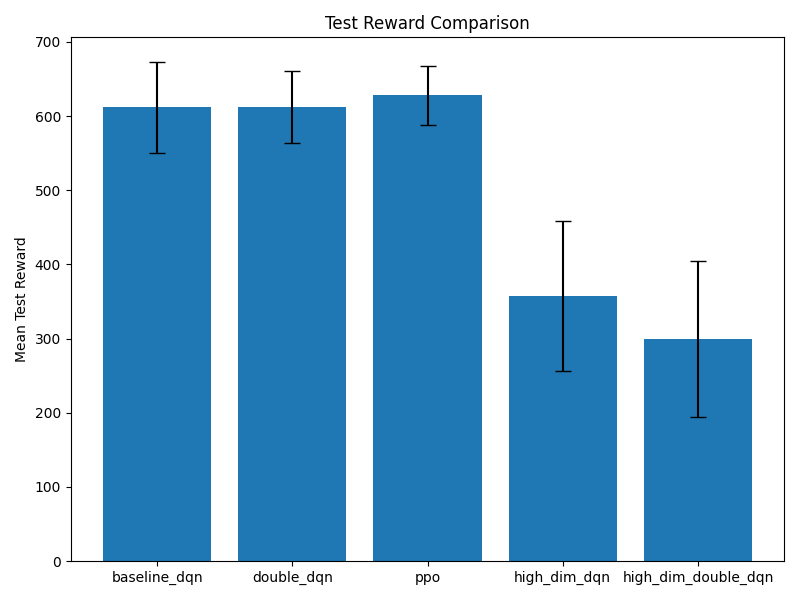
\includegraphics[width=\columnwidth]{images/current_comparison_test_scores.png}
\caption{Mean test reward comparison. Error bars show one standard deviation across 20 test episodes.}
\label{fig:test-score}
\end{center}
\vskip -0.15in
\end{figure}

\subsection{Training Dynamics}

\cref{fig:training} shows the moving-average training reward. PPO improves fastest and avoids the very large negative early returns observed in the high-dimensional value-based agents. DQN and Double DQN both recover from poor early exploration and converge to a similar reward range. The high-dimensional agents start with much lower rewards and recover more slowly, which is consistent with their larger composite action space.

\begin{figure}[t]
\vskip 0.1in
\begin{center}
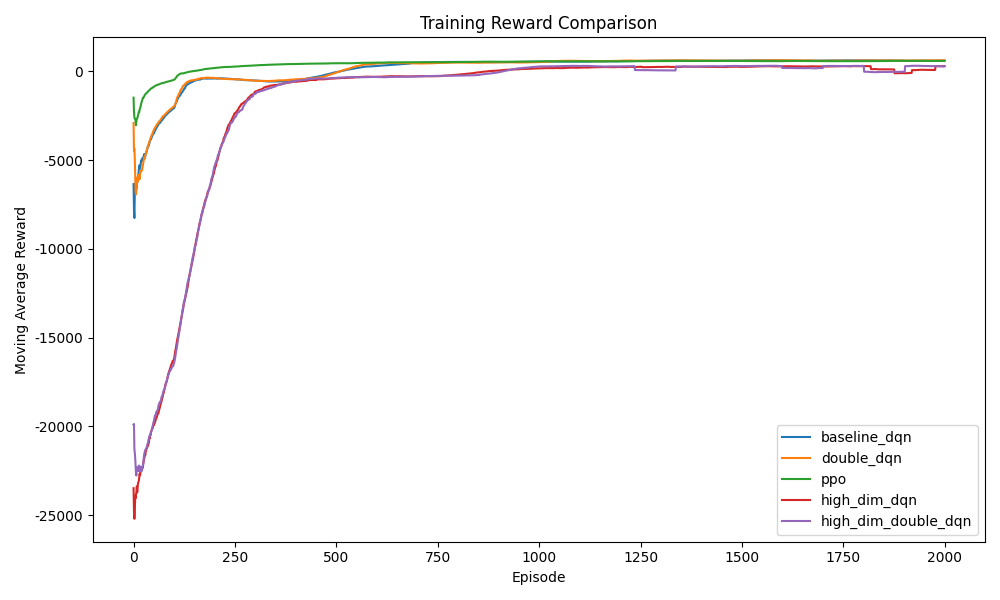
\includegraphics[width=\columnwidth]{images/current_comparison_training_curve.png}
\caption{Training reward moving average for the latest complete runs.}
\label{fig:training}
\end{center}
\vskip -0.15in
\end{figure}

\subsection{Inventory and Ordering Behavior}

\cref{fig:behavior} compares average inventory, order quantity, and unsatisfied demand during testing. All methods draw down the initial inventory quickly and then operate near a lower steady inventory band. PPO and DQN maintain strong demand satisfaction, while Double DQN uses slightly lower average inventory and order quantity at the cost of a lower satisfaction rate. The high-dimensional agents keep higher inventory on average but still do not convert this into higher reward, indicating that the extra action dimensions currently introduce cost and exploration difficulty rather than useful order allocation.

\begin{figure}[t]
\vskip 0.1in
\begin{center}
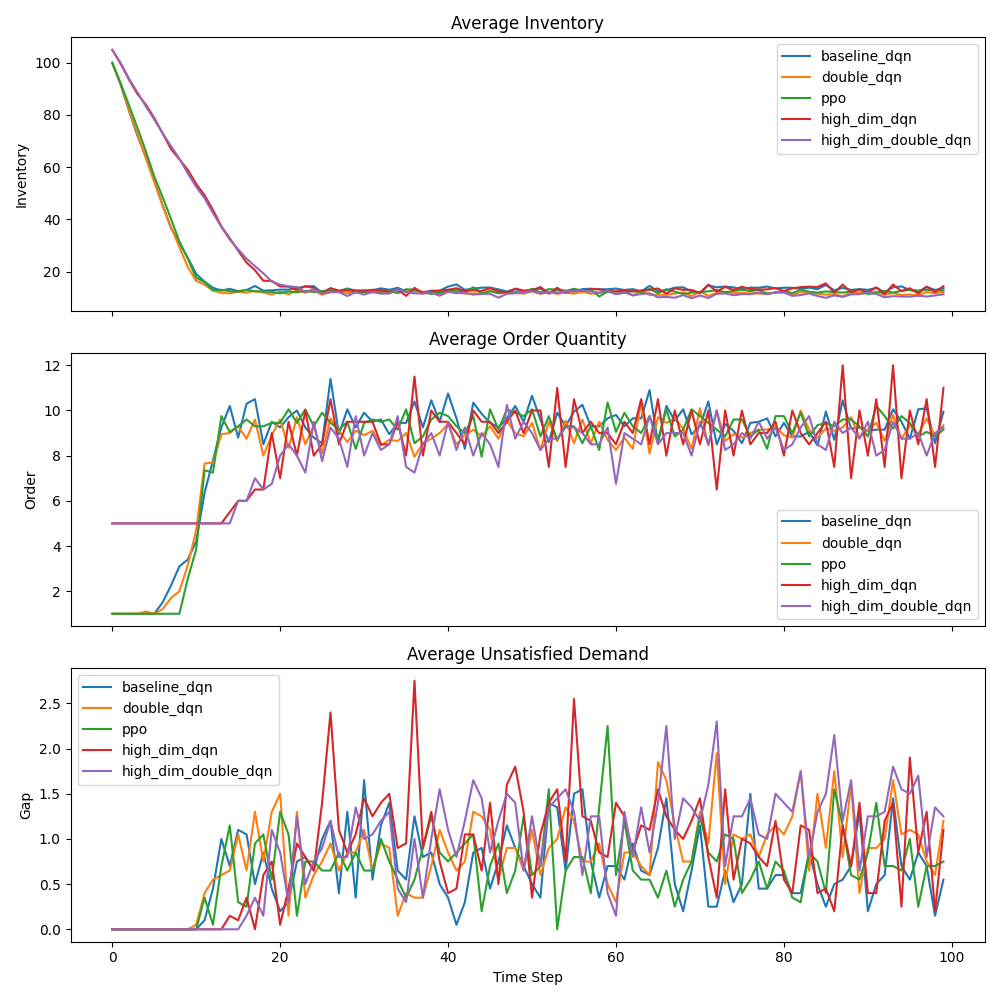
\includegraphics[width=\columnwidth]{images/current_comparison_behavior.png}
\caption{Average inventory, order quantity, and unsatisfied demand during testing.}
\label{fig:behavior}
\end{center}
\vskip -0.15in
\end{figure}

\subsection{High-Dimensional Results}

\cref{tab:highdim-results} reports the latest high-dimensional runs with the same 2000-episode training budget and learning rate $5\times10^{-4}$. High-Dim DQN outperforms High-Dim Double DQN in mean reward, satisfaction rate, and reward variance. This is different from the earlier 1500-episode exploratory High-Dim Double DQN run, which reached a mean reward of 406.10 with learning rate $10^{-3}$. The discrepancy shows that the high-dimensional setting is sensitive to optimization settings and random stream choices.

\begin{table}[t]
\caption{High-dimensional action test performance over 20 test episodes.}
\label{tab:highdim-results}
\vskip 0.15in
\begin{center}
\begin{small}
\begin{tabular}{lcc}
\toprule
Metric & High-Dim DQN & High-Dim Double DQN \\
\midrule
Mean reward & \textbf{357.75} & 299.50 \\
Reward std. & \textbf{100.91} & 104.83 \\
Avg. inventory & 21.73 & \textbf{20.54} \\
Avg. order & 8.43 & \textbf{8.06} \\
Satisfied demand & \textbf{9.28} & 8.94 \\
Demand satisfaction & \textbf{0.917} & 0.904 \\
\bottomrule
\end{tabular}
\end{small}
\end{center}
\vskip -0.1in
\end{table}

\begin{table}[t]
\caption{Additional high-dimensional exploratory runs currently present in \texttt{results/}.}
\label{tab:extra-highdim}
\vskip 0.15in
\begin{center}
\begin{scriptsize}
\begin{tabular}{lcccc}
\toprule
Algorithm & Run & Train eps. & LR & Mean reward \\
\midrule
High-Dim DQN & \texttt{162220} & 1500 & $10^{-3}$ & 351.70 \\
High-Dim Double DQN & \texttt{163325} & 1500 & $10^{-3}$ & \textbf{406.10} \\
\bottomrule
\end{tabular}
\end{scriptsize}
\end{center}
\vskip -0.1in
\end{table}

\section{Discussion}

The main current conclusion is that PPO is the strongest standard-action method in the saved experiments. It achieves the best mean reward, the lowest variance, and a high demand satisfaction rate. Its advantage is not caused by much higher average ordering: its average order quantity is between DQN and Double DQN, suggesting a better balance between inventory protection and holding cost.

Double DQN does not clearly beat DQN in mean reward in the current scalar setting. However, it reduces test-reward variance from 60.96 to 48.61 and uses lower average inventory, so its value is mostly risk reduction and leaner inventory behavior. This is a more conservative conclusion than the previous report, where older results overstated the mean-performance gain of Double DQN.

The high-dimensional formulation is currently not competitive with scalar-action agents. Although it can represent richer order allocation, the composite action space makes exploration harder and increases value-estimation variance. The latest high-dimensional agents preserve demand satisfaction around 0.90--0.92, but their rewards are much lower because higher inventory and unstable orders increase cost. The earlier High-Dim Double DQN run with learning rate $10^{-3}$ suggests there is room for tuning, but the current evidence is not strong enough to claim that the high-dimensional extension improves performance.

\section{Recommendations}

Future training should prioritize three changes. First, repeat each algorithm over multiple seeds and report confidence intervals; the current results are single-run comparisons and should not be interpreted as statistically final. Second, keep PPO as the main standard-action baseline and tune it around entropy coefficient, clip range, and reward scaling. Third, redesign the high-dimensional policy to avoid enumerating all composite actions. A factorized policy or autoregressive order allocator would better match the multi-channel structure and reduce exploration difficulty.

For experiment management, the current Hydra-based layout should be retained. Each run already saves runtime metadata, resolved configuration, logs, model files, scores, and summaries under timestamped \texttt{results/<algorithm>/} directories. The report should continue to state exactly which run directories are used, because the plotting script selects the latest complete run by algorithm name unless explicit result paths are supplied.

\section{Conclusion}

Using the current saved results, PPO is the best-performing standard-action reinforcement learning policy for the Beer Game inventory-control task, with mean reward 627.90 and standard deviation 39.30. DQN and Double DQN have almost identical mean reward, but Double DQN is more stable. The high-dimensional action agents are not yet competitive: their richer action representation increases difficulty and produces substantially lower rewards in the latest comparable runs. The next experimental step should be multi-seed evaluation and targeted tuning of PPO and high-dimensional action factorization.

\end{document}
